\documentclass[a4paper]{scrartcl}
\usepackage[english]{babel}
\usepackage[utf8]{inputenc}
\usepackage{booktabs}
\usepackage{float}
\usepackage{hyperref} 
\usepackage{graphicx}
\usepackage{listings}
\usepackage[style=ieee]{biblatex}
\usepackage{subcaption}
\usepackage{todonotes}

\addbibresource{bibliography.bib}

\renewbibmacro*{bbx:savehash}{}
%----------------------------------------------------------------------------------------
%	TITLE SECTION
%----------------------------------------------------------------------------------------
\title{Traffic-dependent routing based on OpenStreetMap data and TMC messages}

\author{
  Jan Strauß\\
  Matr.-Nr. 2727381\\
  swt85730@stud.uni-stuttgart.de
}

\date{}
%----------------------------------------------------------------------------------------
\begin{document}
\maketitle

\abstract{
In this report a routing application that uses data from the OpenStreetMap project and Traffic Message Channel (TMC) messages to provide traffic-dependent routing on a web-based user interface is presented. This application was developed within the context of the \textit{Fachpraktikum: Algorithms for OpenStreetMap data} course during the summer semester 2016 at the University of Stuttgart.}

%----------------------------------------------------------------------------------------
%	ARTICLE CONTENTS
%----------------------------------------------------------------------------------------
\section{Introduction}
Participants of the course \textit{Fachpraktikum: Algorithms for OpenStreetMap data} were tasked to build a routing application that uses OpenStreetMap \cite{osm_main} data to provide distance and time based routing for cars, bikes and pedestrians. After this base task was completed, the routing application should be extended. \todo{...}

The Implementation presented in \cite{sanwald2013} is written in Java, while the application presented in this report is written in Rust \cite{rust_main}, a new system programming language with strong guarantees on memory and thread safety. The language fits the requirements for a routing application very well: It is a compiled language that offers performance on-par with C++, the standard library contains easy to work with collection types and the language ecosystem offers libraries that provide needed features like a Http server or a parser for pbf files (the OpenStreetMap data format). For a more in-depth discussion see section \ref{impl}.

The remainder of this report is structured as followed: First, the OpenStreetMap data format and TMC concepts are presented in section \ref{bg}. In the next section, \ref{sys}, the system is presented and in section \ref{impl} some implementation details are presented. Finally a conclusion and possible future work is presented in section \ref{concl}

\section{Background}
\label{bg}
\subsection{OpenStreetMap (OSM)}

\todo{ pbf format, ways, nodes, relations, tags}

\subsection{Traffic Message Channel (TMC)}

\todo{ LCL, ECL, DIR, EXT, ... }

\section{System}
\label{sys}

\todo{ general overview (arch diagram)}

\subsection{Parsing OSM data}

\todo{ parsing rounds, conversion, offset, }

\subsection{Routing data representation}
\todo{ structs}

\subsection{Route calculation}

\todo{ Dijkstra, cost method, ...}

\subsection{TMC handling}
\todo{ during osm parsing, extract lc - edge id map and lc,dir - nlc map
during runtime start rdsd, start rdsquery, read input, build event, update maps, handle timeout..}


\subsection{User interface}
\todo{ Static content served from /web directory 
will call /api endpoints 
map is rendered by leaflet }


\begin{figure}[t]
\centering
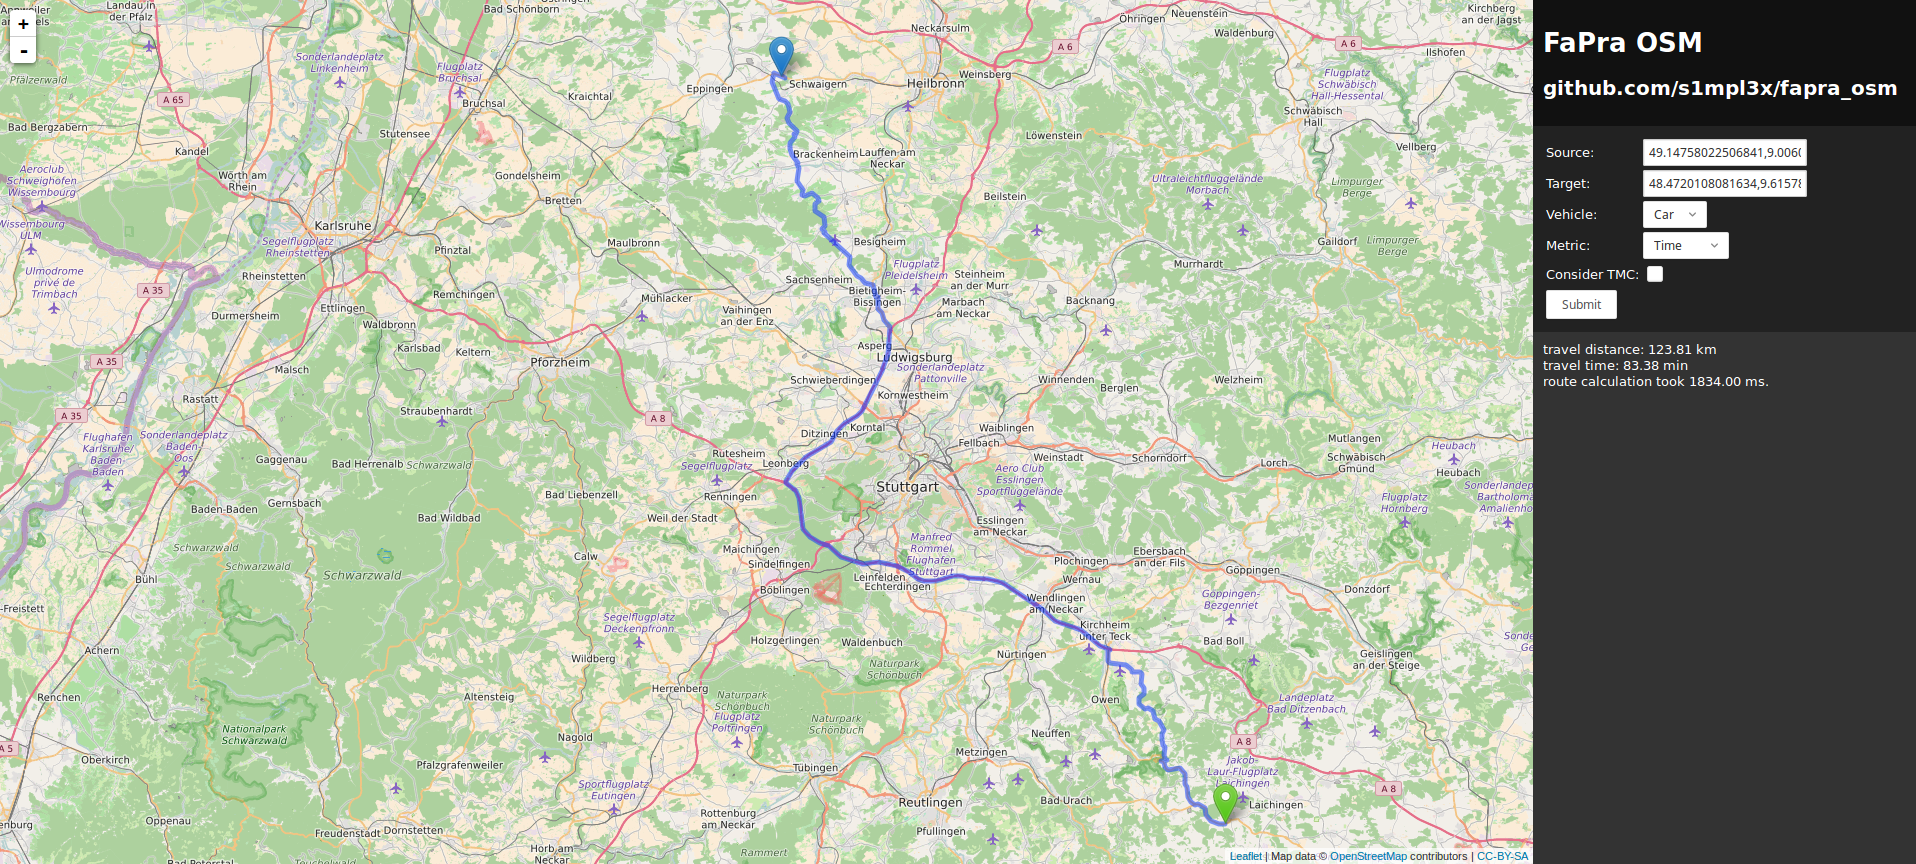
\includegraphics[width=1.0\columnwidth]{img/screenshot.png}
\caption{Web-based graphical user interface}
\label{gui}
\end{figure}

\begin{figure}
    \centering
    \begin{subfigure}[b]{0.4\textwidth}
        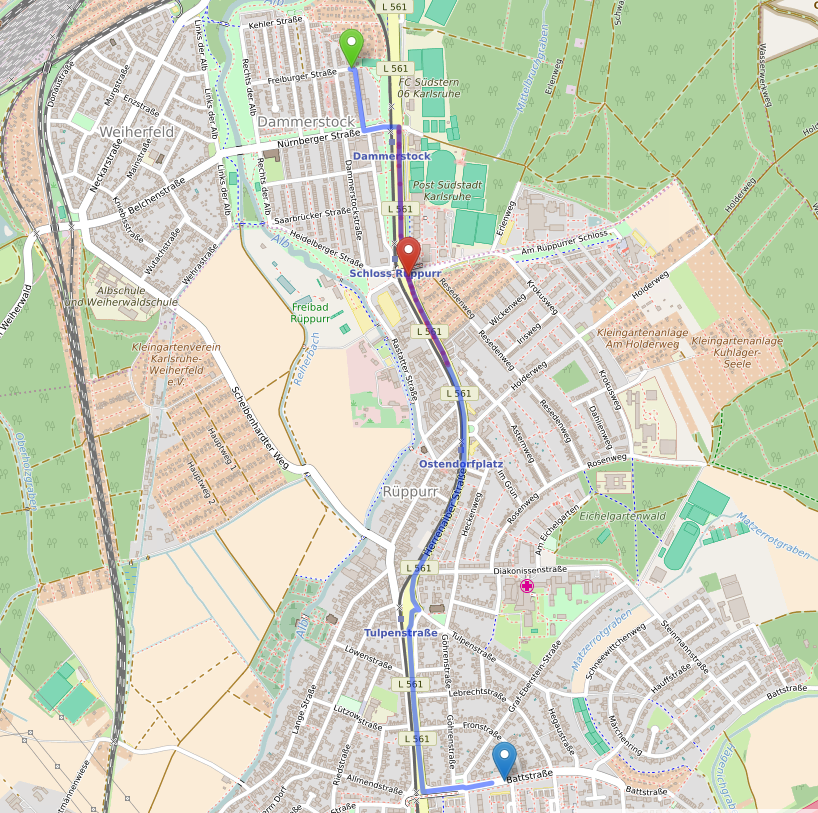
\includegraphics[width=\textwidth]{img/no_tmc.png}
        \caption{Ignoring TMC Events in the route calculation.}
        \label{fig:no_tmc}
    \end{subfigure}
    ~ %add desired spacing between images, e. g. ~, \quad, \qquad, \hfill etc. 
      %(or a blank line to force the subfigure onto a new line)
    \begin{subfigure}[b]{0.4\textwidth}
        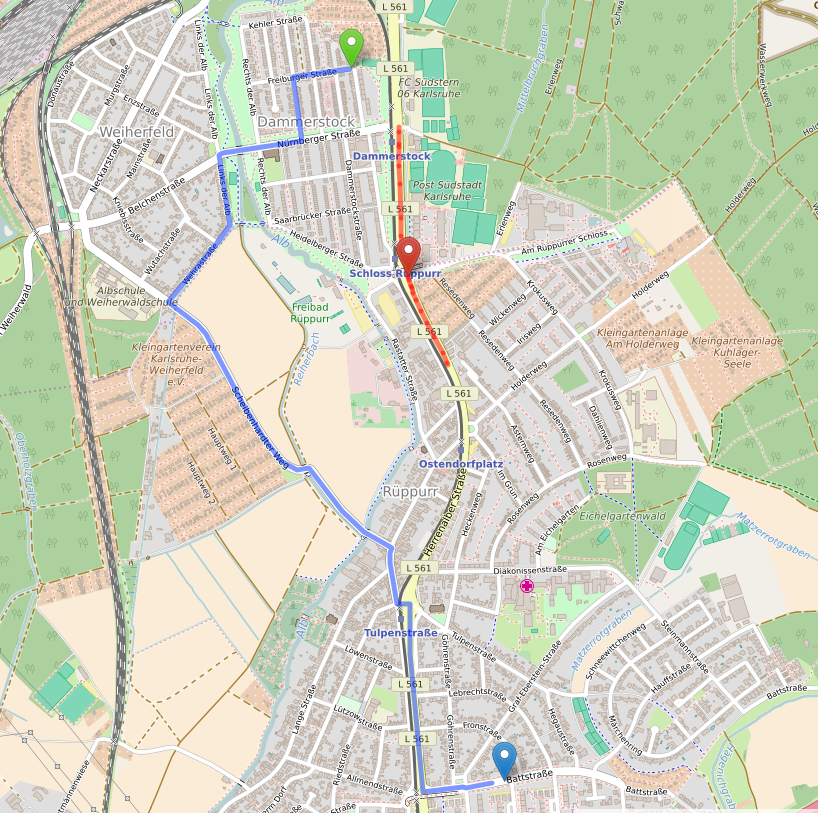
\includegraphics[width=\textwidth]{img/with_tmc.png}
        \caption{Respecting TMC Events in the route calculation.}
        \label{fig:with_tmc}
    \end{subfigure}
    \caption{Effect of respecting TMC events in the route calculation on the shortest found route for the same start and end points.}\label{fig:tmc_comp}
\end{figure}

\section{Implementation}
\label{impl}
\todo{...}

2753 lines of Rust code and about 200 lines of HTML, CSS and JavaScript for the UI\footnote{counted with CLOC \cite{cloc}}

\subsection{Comparision with \citetitle{sanwald2013}}
\todo{ Lang: Java vs. Rust
OSM: relation tags vs. new tagging scheme \cite{osm_wiki_tmc_new_scheme} 
Routing: modify graph (node delay) vs. store in edge-id - delay map

Different interface, binary file format vs text format, parses LCL and ECL, only ECL (similar delay calc)}

\subsection{Used third party libraries/software}
Rust libraries:
Iron \cite{iron}
Iron-staticfile \cite{iron_staticfile}
Iron-mount \cite{iron_mount}
osmpbfreader \cite{osmpbfreader}
rustc-serialize \cite{rustc-serialize}
flate2 \cite{flate2}
bincode \cite{bincode}

Web libraries:
leaflet\cite{leaflet}
jquery \cite{jquery}

\subsection{License and source code}
The source code of the presented application is available at \cite{github} and is licensed under the MIT-License.

\section{Conclusion and future work}
\label{concl}
In this report an application was presented that provides traffic-dependent routing. OpenStreetMap data is used as the base for the routing graph and TMC messages are used as source of current traffic information. While the application works reliably, there are several areas where improvement is possible: The parsing could be sped up by using concurrency, The coverage of TMC events could be improved and cache locality could be increased by storing nodes and edges of the graph in the built grid. 


A major limiting factor is the sparse coverage of TMC tags in the OSM data. Out of 1457361 ways in the Baden-Württemberg extract, only 2666 contained a TMC tag. In the OSM Wiki it is stated that 2906 of 3226 TMC Objects in Baden-Württemberg are tagged \cite{osm_wiki_tmc}, however it is unclear how dated that information is. Due to this fact, the majority of received TMC messages are ignored as they can't be mapped to edges in the routing graph. 


The Rust programming language proved to be suited for building this application, only the compile times and limited tooling support are minor negative points.

%----------------------------------------------------------------------------------------
\printbibliography
%----------------------------------------------------------------------------------------
\end{document}
